\documentclass[tikz,border=2pt,11pt]{standalone}
\usetikzlibrary{arrows.meta}
\usetikzlibrary{positioning}
\usepackage{amsmath}
\usepackage{amssymb}
\usepackage{xcolor}
\usepackage{tikz}
\newcommand{\Q}{\mathbb Q}
\newcommand{\Z}{\mathbb Z}
\newcommand{\R}{\mathbb R}
\newcommand{\C}{\mathbb C}
\newcommand{\F}{\mathbb F}
\newcommand{\Qbar}{\overline{\mathbb Q}}
\newcommand{\Kzero}{K_0}
\newcommand{\Cw}{C_w}
\DeclareMathOperator{\End}{End}
\DeclareMathOperator{\Hom}{Hom}
\DeclareMathOperator{\Tr}{Tr}
\DeclareMathOperator{\Fil}{Fil}
\DeclareMathOperator{\Res}{Res}
\DeclareMathOperator{\GSp}{GSp}
\DeclareMathOperator{\GL}{GL}
\DeclareMathOperator{\SL}{SL}
\DeclareMathOperator{\SU}{SU}
\DeclareMathOperator{\MT}{MT}
\DeclareMathOperator{\Lef}{Lef}
\DeclareMathOperator{\NS}{NS}
\DeclareMathOperator{\Gal}{Gal}
\DeclareMathOperator{\id}{id}
\DeclareMathOperator{\Spec}{Spec}
\begin{document}
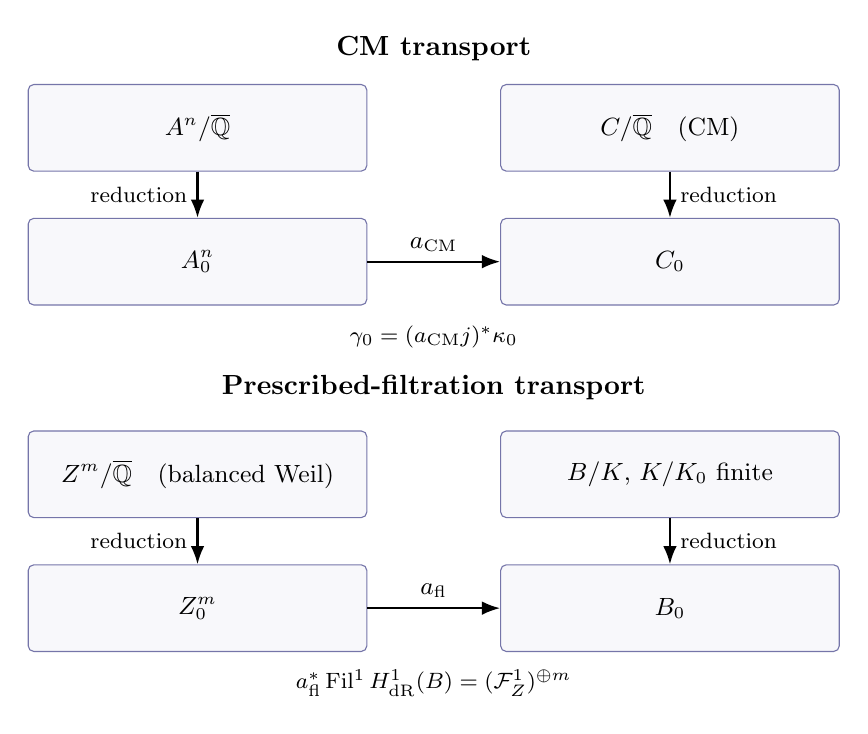
\begin{tikzpicture}[
 >=Latex, font=\small,
 variety/.style={draw=MidnightBlue!60,rounded corners=2pt,
                 fill=MidnightBlue!3,align=center,minimum width=43mm,
                 minimum height=11mm},
 every edge/.style={draw,->,thick},
 note/.style={font=\footnotesize,align=center}]
\node[font=\bfseries] at (3,1.0) {CM transport};
\node[variety] (A) at (0,0) {$A^n/\Qbar$};
\node[variety] (C) at (6,0) {$C/\Qbar$\quad(CM)};
\node[variety] (A0) at (0,-1.7) {$A_0^n$};
\node[variety] (C0) at (6,-1.7) {$C_0$};
\path (A) edge node[left,note] {reduction} (A0);
\path (C) edge node[right,note] {reduction} (C0);
\path (A0) edge node[above] {$a_{\mathrm{CM}}$} (C0);
\node[note] at (3,-2.65) {$\gamma_0=(a_{\mathrm{CM}}j)^*\kappa_0$};
\node[font=\bfseries] at (3,-3.3) {Prescribed-filtration transport};
\node[variety] (Z) at (0,-4.4) {$Z^m/\Qbar$\quad(balanced Weil)};
\node[variety] (B) at (6,-4.4) {$B/K$, $K/K_0$ finite};
\node[variety] (Z0) at (0,-6.1) {$Z_0^m$};
\node[variety] (B0) at (6,-6.1) {$B_0$};
\path (Z) edge node[left,note] {reduction} (Z0);
\path (B) edge node[right,note] {reduction} (B0);
\path (Z0) edge node[above] {$a_{\mathrm{fl}}$} (B0);
\node[note] at (3,-7.05)
 {$a_{\mathrm{fl}}^*\Fil^1H^1_{\mathrm{dR}}(B)
       =(\mathcal F_Z^1)^{\oplus m}$};
\end{tikzpicture}
\end{document}
